% to run it in console: pdflatex main.tex && makeglossaries main && pdflatex main.tex // second for acronyms & glossaries
% also bibtex main -- for bibtex 
% pdflatex -> bibtex + or makeglossaries -> pdflatex
% pdflatex -shell-escape main.tex


%!TEX root = main.tex
\documentclass[a4paper,11pt]{report} %размер бумаги устанавливаем А4, шрифт 12пунк
\usepackage[T1]{fontenc} 
\usepackage{mathptmx} % times new roman
\usepackage[utf8]{inputenc}%включаем свою кодировку: koi8-r или utf8 в UNIX, cp1251 
\usepackage[toc, acronym]{glossaries}
 
\usepackage[english]{babel}%используем русский и английский языки с переносами
\usepackage{amssymb,amsfonts,amsmath,mathtext,cite,enumerate,float} 
\usepackage[unicode]{hyperref} % to make ref clickable
\usepackage{graphicx} %хотим вставлять в диплом рисунки?
% \usepackage{epstopdf}
% \usepackage[dvips]{graphicx} % not working .. image is hidden


\graphicspath{{images/intro/}}%путь к рисункам

\usepackage{geometry} % Меняем поля страницы
% \addtolength{\hoffset}{2.5mm} % shift all text
\geometry{left=2.5cm}% левое поле; 30 mm should be
\geometry{right=2.5cm}% правое поле; 30 mm should be
\geometry{top=2.5cm}% верхнее поле; 38 mm should be 
\geometry{bottom=2.5cm}% нижнее поле; 38mm should be

\renewcommand{\baselinestretch}{1.8} 


\renewcommand{\theenumi}{\arabic{enumi}}% Меняем везде перечисления на цифра.цифра
\renewcommand{\labelenumi}{\arabic{enumi}}% Меняем везде перечисления на цифра.цифра
\renewcommand{\theenumii}{.\arabic{enumii}}% Меняем везде перфра.цифра
\renewcommand{\labelenumii}{\arabic{enumi}.\arabic{enumii}.}% Мена цифра.цифра
\renewcommand{\theenumiii}{.\arabic{enumiii}}% Меняем везцифра.цифра
\renewcommand{\labelenumiii}{\arabic{enumi}.\arabic{enumii}.\arabic{enumiii}.}
\usepackage{cite} % clever references


\usepackage{afterpage}

\newcommand\blankpage{%
    \null
    \thispagestyle{empty}%
    \addtocounter{page}{-1}%
    \newpage}


\usepackage{setspace} % to manpulate spacing
\usepackage{indentfirst} %делать отступ в начале параграфа
\usepackage{enumerate}  %создание и автоматическая нумерация списков
\usepackage{tabularx}  %продвинутые таблицы
\usepackage{tocvsec2} % for settocdepth; diffrent level of depth
\settocdepth{subsection} % for all document; section, subsection & co

\makeatletter
\def\@makechapterhead#1{%
  \vspace*{50\p@}% <----------------- Space from top of page to Chapter #
  {\parindent \z@ \raggedright \normalfont
    \ifnum \c@secnumdepth >\m@ne
        \huge\bfseries \thechapter.\ % <-- Chapter # (without "Chapter")3
    \fi
    \interlinepenalty\@M
    #1\par\nobreak% <------------------ Chapter title
    \vskip 30\p@% <------------------ Space between chapter title and first paragraph
  }}
\makeatother

% \renewcommand{\thechapter}{\Roman{chapter}}

\usepackage[titletoc]{appendix}

% \usepackage{titlesec}  % to remove chapter name
% \titleformat{\chapter}[display]
%   {\Huge\bfseries}
%   {}
%   {0pt}
%   {\thechapter.\ }

% \titleformat{name=\chapter,numberless}[display]
%   {\Huge\bfseries}
%   {}
%   {0pt}
%   {}

\setcounter{secnumdepth}{3} % to numerate subsection -- 3;


\usepackage[nottoc]{tocbibind}

\makeglossaries
\newglossaryentry{latex}
{
        name=latex,
        description={Is a mark up language specially suited for 
scientific documents}
}
\newglossaryentry{maths}
{
        name=mathematics,
        description={Mathematics is what mathematicians do}
}
\newglossaryentry{formula}
{
        name=formula,
        description={A mathematical expression}
}
 
\newacronym{gcd}{GCD}{Greatest Common Divisor}
\newacronym{lcm}{LCM}{Least Common Multiple}
 




% Bibtex
% \makeatletter
% \renewcommand{\@biblabel}[1]{#1.} %Заменяем библиографию с квадратных скобок на точку в списке литературы
% \makeatother

% \addcontentsline{toc}{chapter}{}


\begin{document}

\begin{titlepage}


\newpage
\vspace*{1.5cm}
\begin{center}
{\fontsize{22}{26}\selectfont Development of the Single Pixel Based Detector and Telescope}
% FEDERALNOE AGENTSTVO PO OBRAZOVANIJu RF \\
% \vspace{1cm}
% N-SKIJ ARBUZO-LITEJNYJ INSTITUT \\*
% (GOSUDARSTVENNYJ UNIVERSITET) \\*
% \hrulefill
\end{center}

% \flushright{KAFEDRA  HHH}

\vspace{15em}
\begin{center}
{\fontsize{16}{16}\selectfont
Leonov Vladimir 
}
\end{center}

\vspace{10cm}

% \begin{figure}[h]
% \center{
\includegraphics[width=0.75\linewidth]{skku}}
% \vspace{1cm} 
% % \caption{Noise-distance}
% \label{fig:skku} % or change caption location
% \end{figure}



\begin{center}

% \textsc{\textbf{issledovanie torsionnyh nanogeneratorov \linebreak stvolovyh kletok dlja borby s terrorizmom}}
{\setstretch{1}\fontsize{16}{16}\selectfont
The Graduate School \\
Sungkyunkwan University \\
Department of Physics\\
}

\end{center}


\afterpage{\blankpage}

\vspace*{1cm}
\begin{center}
{\fontsize{22}{26}\selectfont Development of the Single Pixel Based Detector and Telescope}
% FEDERALNOE AGENTSTVO PO OBRAZOVANIJu RF \\
% \vspace{1cm}
% N-SKIJ ARBUZO-LITEJNYJ INSTITUT \\*
% (GOSUDARSTVENNYJ UNIVERSITET) \\*
% \hrulefill
\end{center}

% \flushright{KAFEDRA  HHH}

\vspace{15em}
\thispagestyle{empty}
\begin{center}
{\fontsize{16}{16}\selectfont
Leonov Vladimir 
}
\end{center}

\vspace{12cm}

% \begin{figure}[h]
% \center{
\includegraphics[width=0.75\linewidth]{skku}}
% \vspace{1cm} 
% % \caption{Noise-distance}
% \label{fig:skku} % or change caption location
% \end{figure}



\begin{center}
% \textsc{\textbf{issledovanie torsionnyh nanogeneratorov \linebreak stvolovyh kletok dlja borby s terrorizmom}}
{\setstretch{1}\fontsize{16}{16}\selectfont
The Graduate School \\
Sungkyunkwan University \\
Department of Physics\\
}
\end{center}




\afterpage{\blankpage}



\vspace*{1cm}
\begin{center}
{\fontsize{22}{26}\selectfont Development of the Single Pixel Based Detector and Telescope}
\end{center}


\vspace{15em}
\thispagestyle{empty}
\begin{center}
{\fontsize{16}{16}\selectfont
Leonov Vladimir 
}
\end{center}

\begin{center}
{\setstretch{1.5}\fontsize{14}{16}\selectfont
A Master's Thesis Submitted to the Department of Physics \\
and the Graduate School of Sungkyunkwan University \\
in partial fulfillment of the requirements \\
for the degree of Master of Arts in Science\\

\vspace{2cm}

[June 2018]
}



\vspace{4cm}


{\setstretch{1}\fontsize{16}{18}\selectfont
Approved by \\
\vspace{3mm}
Il H. Park, Ph.D. \\
\vspace{3mm}
Major Advisor \\
}

\end{center}


\afterpage{\blankpage}

\begin{center}

\vspace*{2.5cm}
{\setstretch{1}\fontsize{16}{18}\selectfont
This certifies that the master's thesis \\
of Leonov Vladimir is approved
}
\end{center}



\thispagestyle{empty}
\vspace{6cm}

\begin{flushright}
\noindent\rule{7cm}{0.4pt} \\
\vspace{0.6cm}
\noindent\rule{7cm}{0.4pt} \\
\vspace{0.6cm}
\noindent\rule{7cm}{0.4pt} \\
\end{flushright}

\vspace{\fill}


\begin{center}
% \textsc{\textbf{issledovanie torsionnyh nanogeneratorov \linebreak stvolovyh kletok dlja borby s terrorizmom}}
{\setstretch{1}\fontsize{16}{16}\selectfont
The Graduate School \\
Sungkyunkwan University \\
June 2018\\
}
\end{center}

\afterpage{\blankpage}

\end{titlepage}% это титульный лист

 
\begin{spacing}{1.2}
\setcounter{page}{1}
\tableofcontents 
% \addcontentsline{toc}{chapter}{Appendix A} % since nu,ber is removed.
\end{spacing} 
\newpage

% list of tables
\listoftables
% % list of figures
\listoffigures
% % glossary & acronim
\printglossary[type=\acronymtype]
\printglossary

\chapter{Introduction}
% \chapter[Title with Larger Font Size]{\fontsize{18}{5}\selectfont{Title with Larger Font Size}}

\section{General moments}
When using the  and \\chapter tags in LaTeX you will typically end up with parts and chapters that say “part” and “chapter” before the name you have written. Putting these lines in your preamble will remove this:

\label{my_desire}
Hello to everyone, I really want to make
Latex diploma and I will
\subsection{MEMS}
MEMS,Alexander Refsum Jensenius is a music researcher and research musician living in Oslo, Norway Alexander Refsum Jensenius is a music researcher and research musician living in Oslo, Norway
\subsection{SIPM}
MEMS,Alexander Refsum Jensenius is a music researcher and research musician living in Oslo, Norway Alexander Refsum Jensenius is a music researcher and research musician living in Oslo, Norway
MEMS,Alexander Refsum Jensenius is a music researcher and research musician living in Oslo, Norway Alexander Refsum Jensenius is a music researcher and research musician living in Oslo, Norway

MEMS,Alexander Refsum Jensenius is a music researcher and research musician living in Oslo, Norway Alexander Refsum Jensenius is a music researcher and research musician living in Oslo, Norway

MEMS,Alexander Refsum Jensenius is a music researcher and research musician living in Oslo, Norway Alexander Refsum Jensenius is a music researcher and research musician living in Oslo, Norway

MEMS,Alexander Refsum Jensenius is a music researcher and research musician living in Oslo, Norway Alexander Refsum Jensenius is a music researcher and research musician living in Oslo, Norway

MEMS,Alexander Refsum Jensenius is a music researcher and research musician living in Oslo, Norway Alexander Refsum Jensenius is a music researcher and research musician living in Oslo, Norway

MEMS,Alexander Refsum Jensenius is a music researcher and research musician living in Oslo, Norway Alexander Refsum Jensenius is a music researcher and research musician living in Oslo, Norway

MEMS,Alexander Refsum Jensenius is a music researcher and research musician living in Oslo, Norway Alexander Refsum Jensenius is a music researcher and research musician living in Oslo, Norway

MEMS,Alexander Refsum Jensenius is a music researcher and research musician living in Oslo, Norway Alexander Refsum Jensenius is a music researcher and research musician living in Oslo, Norway

MEMS,Alexander Refsum Jensenius is a music researcher and research musician living in Oslo, Norway Alexander Refsum Jensenius is a music researcher and research musician living in Oslo, Norway
MEMS,Alexander Refsum Jensenius is a music researcher and research musician living in Oslo, Norway Alexander Refsum Jensenius is a music researcher and research musician living in Oslo, Norway
MEMS,Alexander Refsum Jensenius is a music researcher and research musician living in Oslo, Norway Alexander Refsum Jensenius is a music researcher and research musician living in Oslo, Norway
MEMS,Alexander Refsum Jensenius is a music researcher and research musician living in Oslo, Norway Alexander Refsum Jensenius is a music researcher and research musician living in Oslo, Norway
MEMS,Alexander Refsum Jensenius is a music researcher and research musician living in Oslo, Norway Alexander Refsum Jensenius is a music researcher and research musician living in Oslo, Norway
MEMS,Alexander Refsum Jensenius is a music researcher and research musician living in Oslo, Norway Alexander Refsum Jensenius is a music researcher and research musician living in Oslo, Norway

MEMS,Alexander Refsum Jensenius is a music researcher and research musician living in Oslo, Norway Alexander Refsum Jensenius is a music researcher and research musician living in Oslo, Norway

MEMS,Alexander Refsum Jensenius is a music researcher and research musician living in Oslo, Norway Alexander Refsum Jensenius is a music researcher and research musician living in Oslo, Norway

MEMS,Alexander Refsum Jensenius is a music researcher and research musician living in Oslo, Norway Alexander Refsum Jensenius is a music researcher and research musician living in Oslo, Norway

asdasd as I said in ~\ref{my_desire}

asd
s

\begin{enumerate}
\item xcxc
\item xc
\item xcx
\end{enumerate}

Table is:
\ref{tbl:test_table}

Fig is:
\ref{fig:test_fig}

\begin{itemize}
\item xcxc
\item xcxc
\item cf
\end{itemize}

\section{general moments \#2}
FPGA, Alexander Refsum Jensenius is a music researcher and research musician living in Oslo, Norway Alexander Refsum Jensenius is a music researcher and research musician living in Oslo, Norway

\chapter{Hardware}
\section{Logic of submodule electronics}

All the logic of the submodule is shown in the figure \ref{fig:submodule_logic}.

\begin{figure}[H]
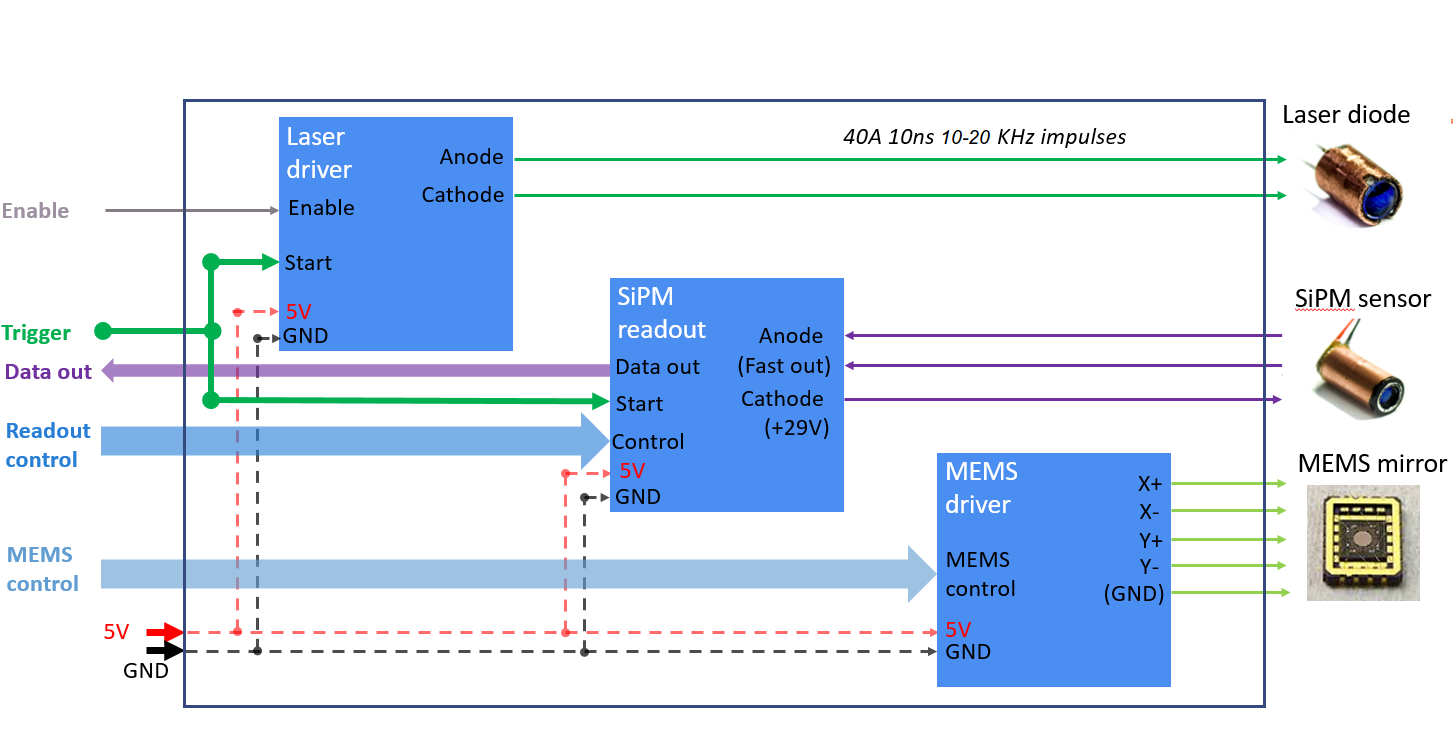
\includegraphics[width=1.05\linewidth]{logic}
\caption{Logic diagram of submodule electronics.}
\label{fig:submodule_logic}
\end{figure}

MEMS driver works independently from other modules, controlling only MEMS mirror. SiPM and Laser driver are joint by trigger signal. Laser driver utilize for shooting of laser diode, SiPM board generating high voltage for SiPM, performs readout and amplification of SiPM signal and measuring time delay between outgoing and return impulse by TDC chip.
Power supply for all components is +5V. Each components are described in detail below.

\subsection{Laser driver logic}
It is very easy to operate a laser diode, in addition to power supply (+5V) of a laser driver, we just need provide LH (Logical High, 3.3V for here) to the Enable input and clock signal with desirable frequency $f$ to the Trigger input, after that Laser driver repeats electrical 40A pulses with 10ns width for Laser diode.

\begin{figure}[H]
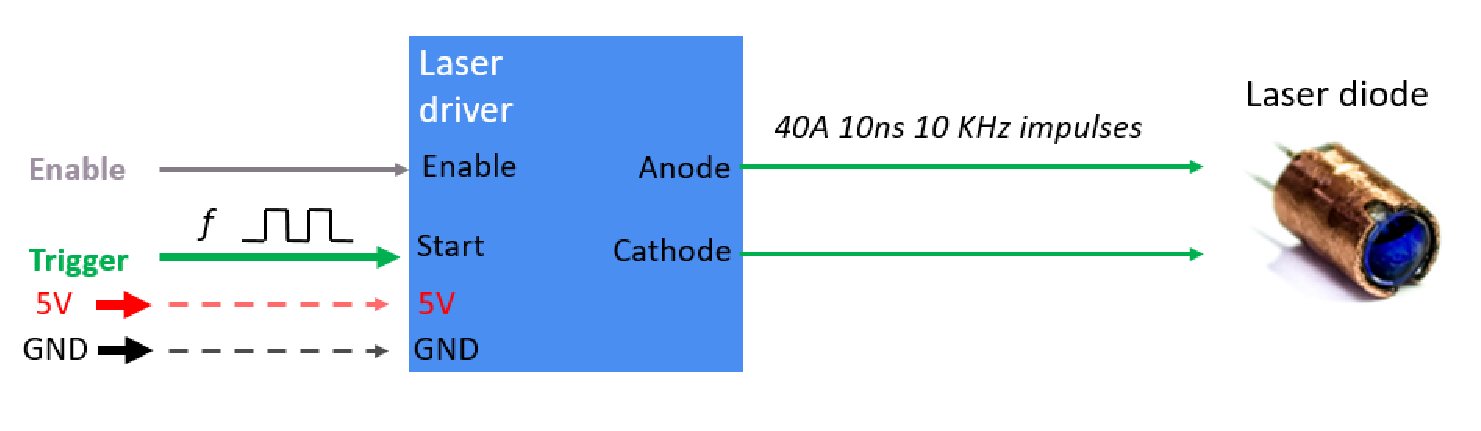
\includegraphics[width=1\linewidth]{ld_logic}
\caption{Logic diagram of laser driver.}
\label{fig:real_submodule}
\end{figure}

\subsection{MEMS driver logic}

MEMS driver board has a power (+5V) and control (SPI) input which are used for the control of MEMS mirror via SPI commands to 16-bit DAC, which produces a high-voltage (160V) 4-channel signal (X+, X-, Y+, Y-). 
We used 16-bit DAC with 20MHz SPI speed. 
Filter clocks input is used for set LPF cutoff frequency, to avoid high frequency which can induce resonance and damage of the mirror.


\begin{figure}[H]
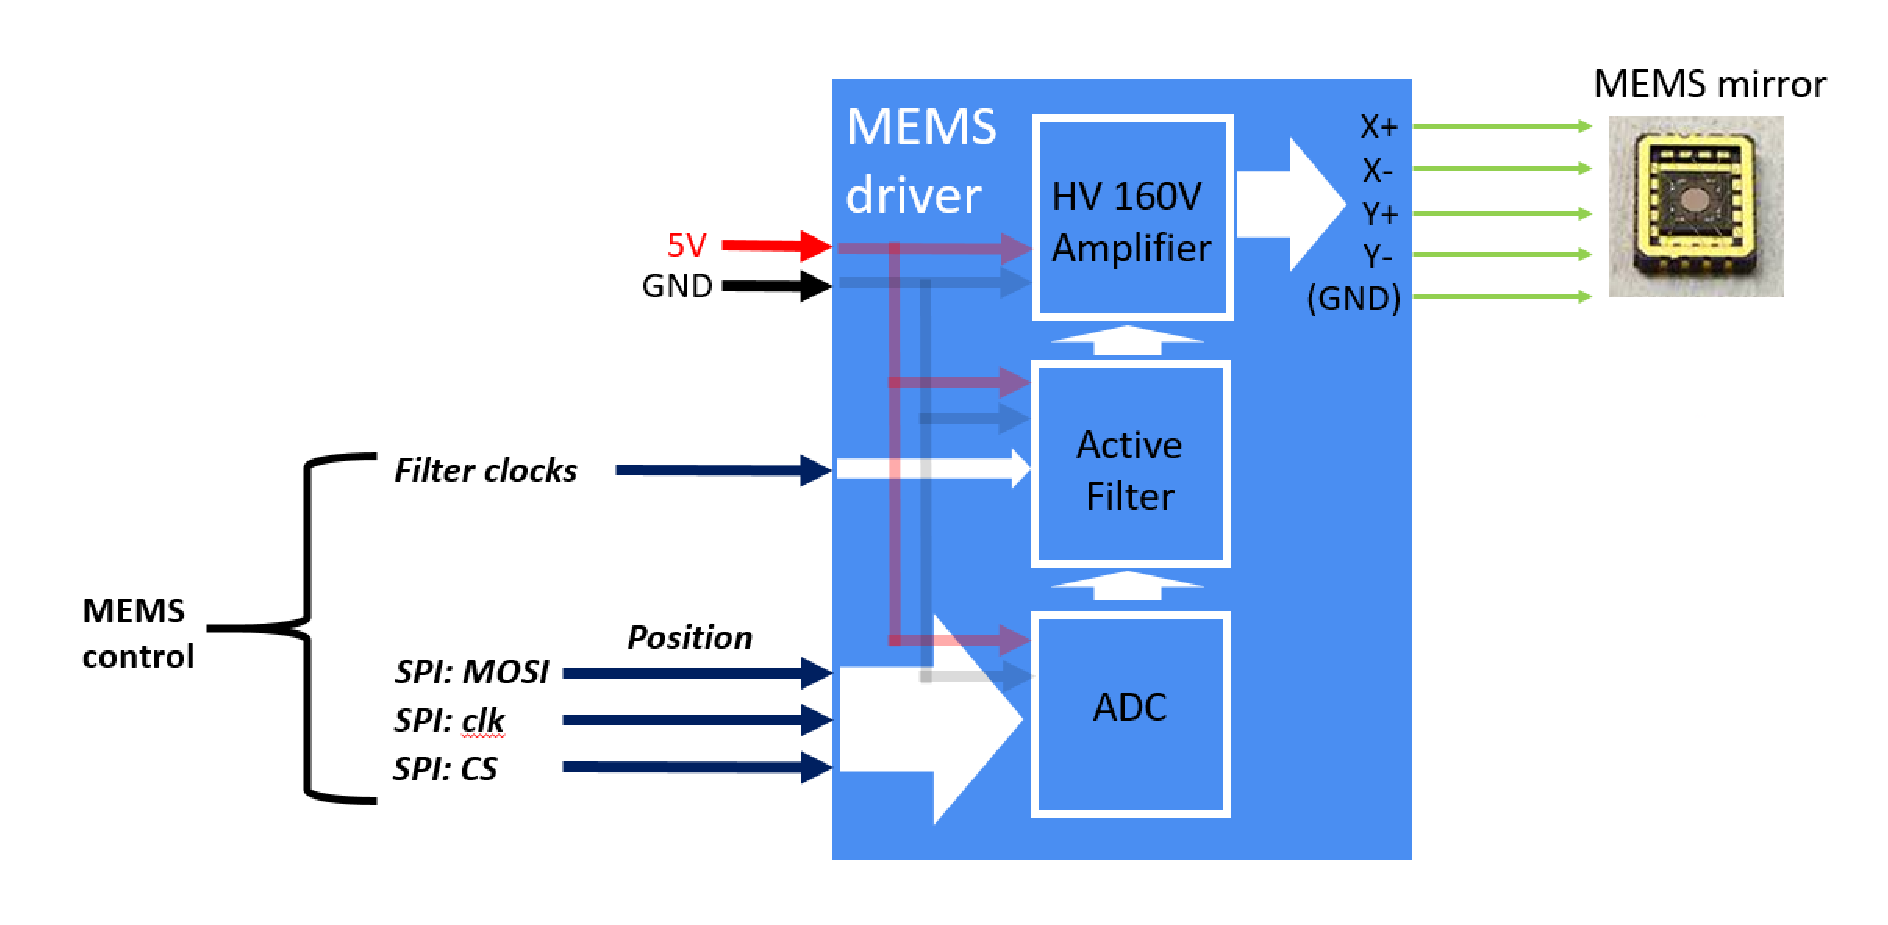
\includegraphics[width=1\linewidth]{mems_logic}
\caption{Logic diagram of MEMS driver.}
\label{fig:real_submodule}
\end{figure}


To form a trajectory with maximum possible FPS, for axis X applied voltage sine and for axis Y applied voltage like pulse with triangle shape. Depending on sine frequency we can get different number of lines, that makes vertical resolution very flexible as shiown in figure \ref{fig:mems_real_trajectories}.



\begin{figure}[H]
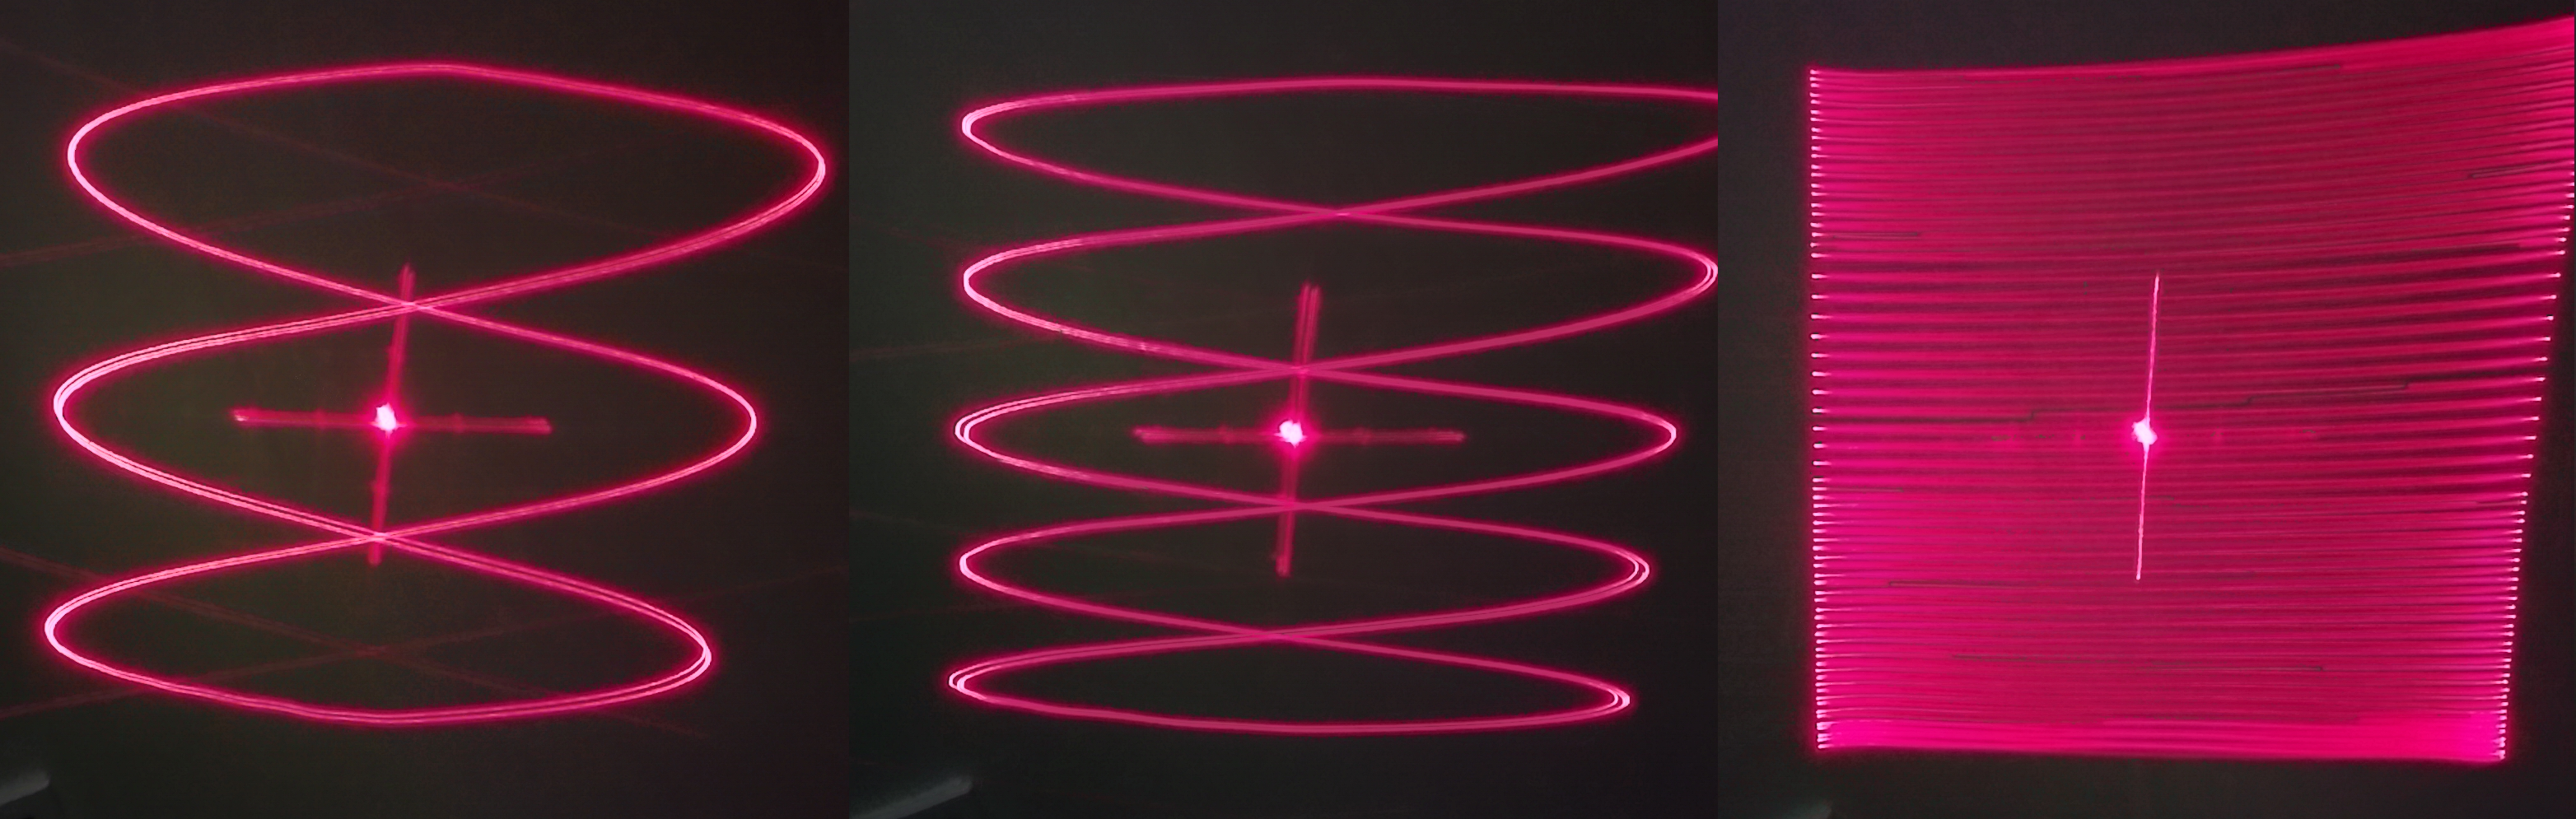
\includegraphics[width=1\linewidth]{mems_real_trajectories}
\caption{Photo of different resolutions: 4,8 and 60 lines.}
\label{fig:mems_real_trajectories}
\end{figure}





\subsection{SiPM logic}

SiPM board has a power (+5V) which is transformed to +29V for SiPM bias voltage and $\pm5 V$ for amplifier voltage. Readout contol (SPI) input are used for the control of TDC.
After aplification of the SiPM output (Fast out), signal goes to comparator, if level exceeds treshold, LH is provided to TDC Stop input.
After that, when TDC finished time calculation, Interrupt pin is fired and the result can be read by SPI DOUT.
Ref clk input is waiting for high frequecy clock signal - 12.5 MHz in our case, which is used for TDC measurement.



\begin{figure}[H]
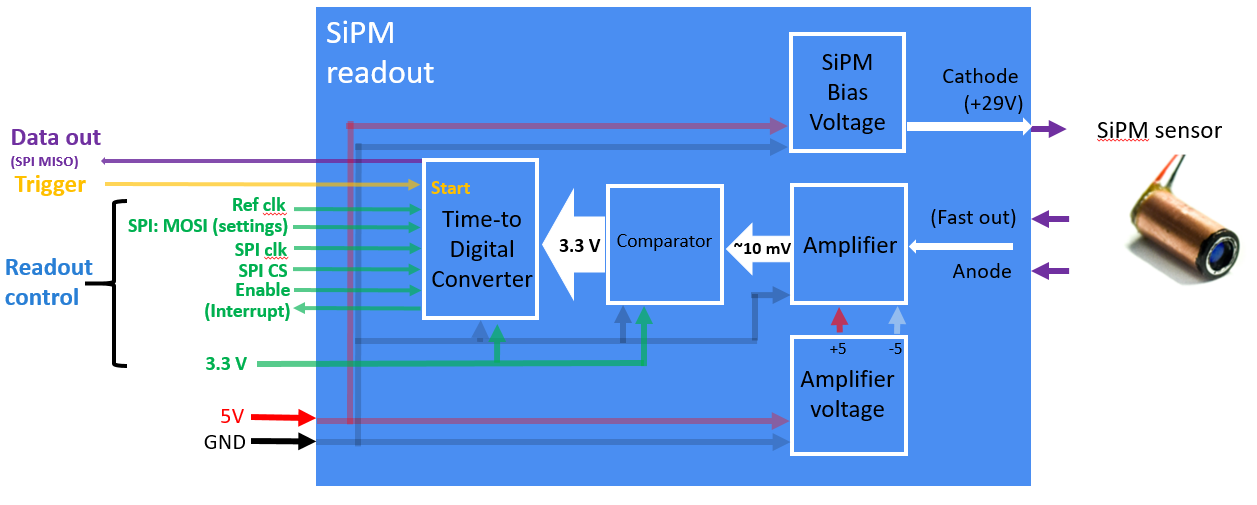
\includegraphics[width=1\linewidth]{sipm_logic}
\caption{Designed and real assembled submodule.}
\label{fig:real_submodule}
\end{figure}


During descring green board also desribe power board

\section{Control board}
In the beginning, logic control was performed by the micro CPU, which allowed to quickly develop a pilot version of the control board. Then, with growing needs, it became obvious the need to use FPGA, giving advantages in speed and parallelism, so the final version of the control board was completely implemented on FPGA.

The clock was modified via PLL from 50 to 64 MHz.
FPGA has faster clock + allow parallel \& less jitter.

\begin{figure}[H]
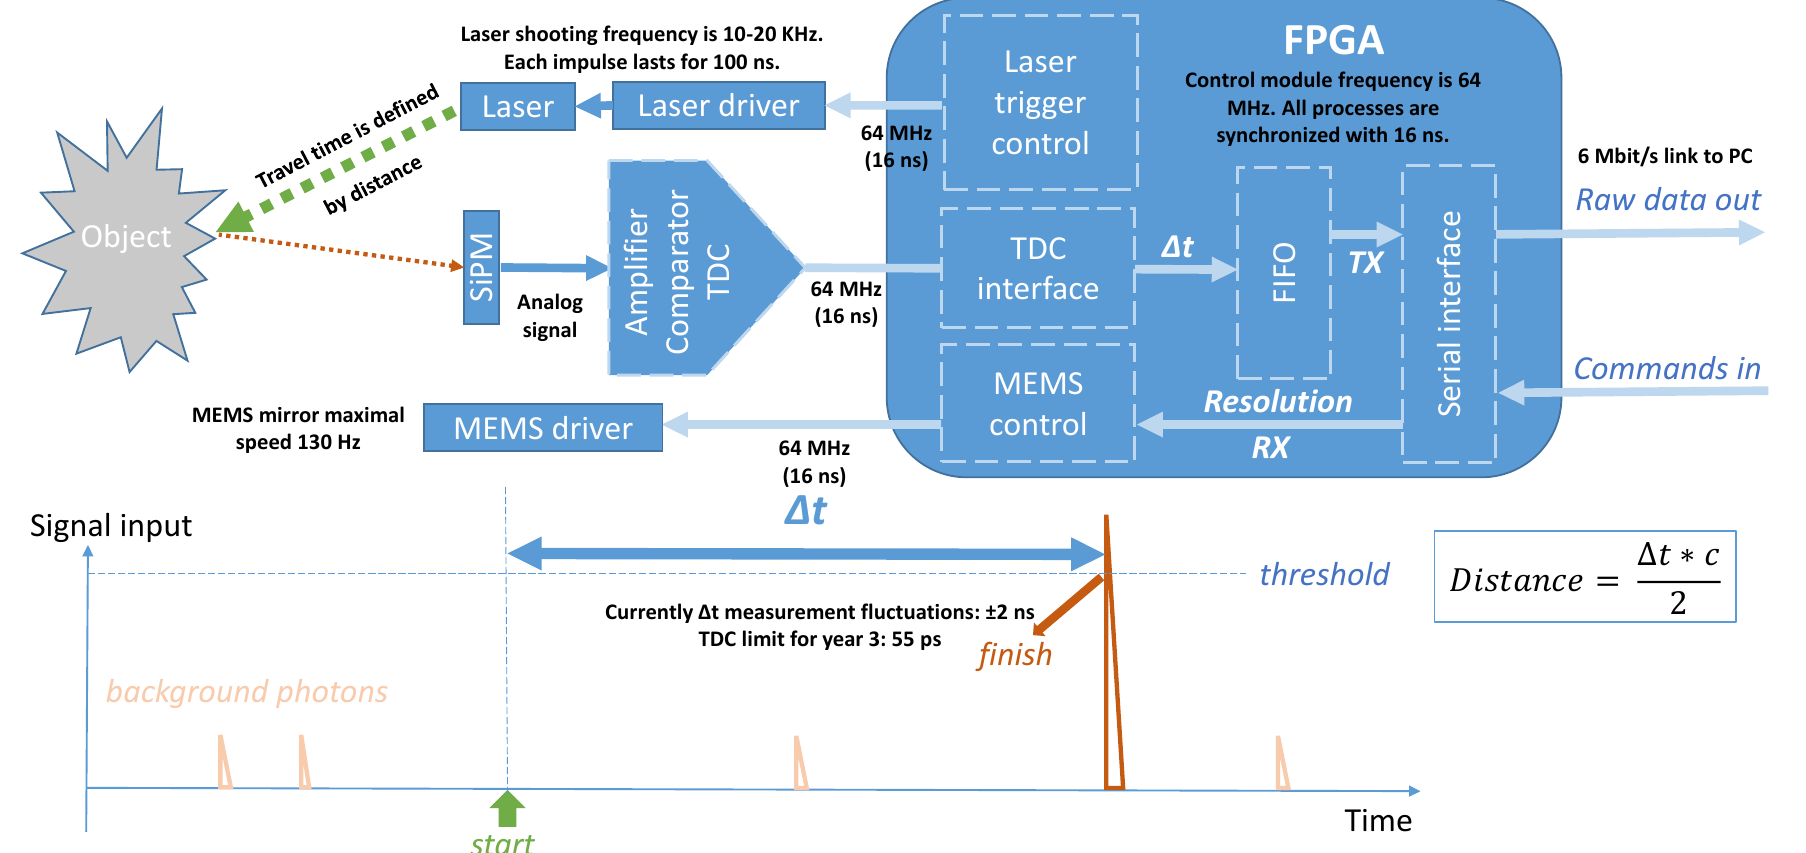
\includegraphics[width=1.1\linewidth]{control}
\caption{Designed and real assembled submodule.}
\label{fig:real_submodule}
\end{figure}



AZAZAZA
Their long-term aid ~\cite{Haggarty:01} ~\cite{Haggarty:02}

The \Gls{latex} typesetting markup language is specially suitable 
for documents that include \gls{maths}. \Glspl{formula} are 
rendered properly an easily once one gets used to the commands.
 
Given a set of numbers, there are elementary methods to compute 
its \acrlong{gcd}, which is abbreviated \acrshort{gcd}. This 
process is similar to that used for the \acrfull{lcm}.

\renewcommand{\bibname}{References}
\bibliographystyle{unsrt}
\bibliography{refs}

% \chapter{Appedix A} % to remove number we use * + this one is needed in the biblio \addcontentsline{toc}{chapter}{Appendix A} 
% \section{azazaz}
% \paragraph{aza}
% % \label{my_desire}
% Hello to everyone, I really want to make
% Latex diploma and I will
% \subsection{sub}
% this is sub..

% \section{azazaz}
% asdasd as I said in ~\ref{my_desire}

% asd
% s

% \begin{enumerate}
% \item xczxc
% \item xdf
% \item fdgf
% \end{enumerate}

% \begin{itemize}
% \item dfdf
% \item sdfs
% \item sdfs
% \end{itemize}

% \section*{azazaz}

\begin{appendices}
  \chapter{Consectetur adipiscing elit}
  \section{First part}
  asxdsdsa
  \section{Second}
  I'm a second part!
  \chapter{Mauris euismod}
  ~\ref{fig:skku}
\end{appendices}
% это титульный лист



\end{document}


